\section{Recurrent Neural Networks (RNNs)}

\begin{frame}\frametitle{\subsecname}

\begin{itemize}
\item Feedforward networks:\\

\underline{Data}:
\begin{equation*}
\Big\{ \left(\vec x^{(\alpha)}, \vec y^{(\alpha)}_{\mathrm{True}} \right) \Big\}\,,\quad \alpha = 1,\ldots,p
\end{equation*}

\pause

\begin{itemize}
\item any two sample pairs $\left(\vec x^{(\alpha)}, \vec y^{(\alpha)}_{\mathrm{True}} \right)$ and $\left(\vec x^{(\alpha')}, \vec y^{(\alpha')}_{\mathrm{True}} \right)$ are assumed to be \iid
\item Their respective predictions $\vec y(\vec x^{(\alpha)}; \vec w)$ and $\vec y(\vec x^{(\alpha')}; \vec w)$ are also independent from one another.
\end{itemize}

\pause

\item RNN \corresponds~Neural network with loops.\\

\underline{Data}:\\

\begin{equation*}
\Big\{ \left(\vec x^{(\alpha,t)}, \vec y^{(\alpha,t)}_{\mathrm{True}} \right)_{t=1}^{n_{\alpha}} \Big\}\,,\quad \alpha = 1,\ldots,p
\end{equation*}

\pause

\begin{itemize}
\item $p$ \iid sequences
\item each sequence $\alpha$ contains $n_{\alpha}$ time steps
\item Use information from the previous step to predict the next step.
\end{itemize}

\end{itemize}

\end{frame}


\subsection{Basic RNN}

\mode<presentation>{

\begin{frame}\frametitle{\subsecname}

\begin{figure}[ht]
     \centering
	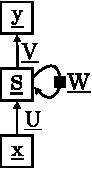
\includegraphics[width=0.2\textwidth]{img/rnn}
     \mode<article>{
	\caption{Basic RNN architecture}
	}
	\label{fig:rnn} 
\end{figure}
\end{frame}
}

\begin{frame}\frametitle{\subsecname}

%Omitting sequence index $\alpha$
\begin{center}

	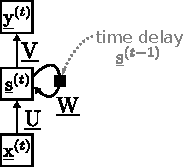
\includegraphics[width=\slidesonly{0.4}\notesonly{0.2}\textwidth]{img/rnn_time_delay}
     \mode<article>{
	\captionof{figure}{Basic RNN architecture}
	}
	\label{fig:rnn_time_delay} 
\end{center}


\end{frame}

\subsubsection{The tunable parameters of a basic RNN}

\definecolor{darkgreen}{rgb}{0,0.6,0}

\begin{frame}\frametitle{\subsubsecname}

\mode<article>{
\begin{center}
	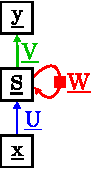
\includegraphics[width=0.1\textwidth]{img/rnn_colored}
     \mode<article>{
	\captionof{figure}{Basic RNN architecture}
	}
	\label{fig:rnn} 
\end{center}
}
\mode<presentation>{
\placeimage{13}{1}{img/rnn_colored}{width=2cm}
}

Let
\begin{itemize}
\item[] $N$ be the number of input variables $\rightarrow$ $\vec x^{(t)} \in \R^N$
\item[] $H$ be the number of hidden nodes
\item[] $M$ be the number of output nodes
\end{itemize}

\pause

\newpage

Identify the free parameters (trainable weights) of the network:

\begin{itemize}
\item input-to-hidden: ${\color{blue} \vec U = (\vec u_1,\ldots, \vec u_i, \ldots,\vec u_H)} \in \R^{H,N}$
\item hidden-to-hidden: ${\color{red} \vec W = (\vec w_1,\ldots, \vec w_j, \ldots,\vec u_H)} \in \R^{H,H}$
\item hidden-to-output: ${\color{darkgreen} \vec V = (\vec v_1,\ldots, \vec v_k, \ldots,\vec v_H)} \in \R^{M,H}$
\end{itemize}




\end{frame}

\begin{frame}\frametitle{Weight matrices in basic RNN}
Remark: The weight matrices are constructed slightly differently than how we defined them for MLPs. We now stack \textbf{row} vectors instead of \textbf{column} vectors.\\
Reason: brevity, to avoid putting transpose everywhere

\begin{itemize}
\only<1>{
\item input-to-hidden:\\

The weights from each input $x_j$ to each hidden node $h_i$:
\begin{equation}
\vec u_i = ( u_{i1},\ldots,  u_{ij}, \ldots, u_{iN}) \text{ with } j=1,\ldots,N \text{ and } i=1,\ldots,H
\end{equation}

\begin{equation}
\vec U = 
\left(
\begin{array}{ccc}
  \horzbar & \vec u_1 &  \horzbar \\
  \horzbar & \vec u_2 &  \horzbar \\
		   & \vdots    &          \\
  \horzbar & \vec u_H &  \horzbar
\end{array}
\right) \in \R^{H,N}
\end{equation}
}
\only<2>{
\item hidden-to-hidden:\\

The weights to each hidden node $h_i$:
\begin{equation}
\vec w_i = ( w_{i1},\ldots,  w_{ij}, \ldots, w_{iH}) \text{ with } i,j=1,\ldots,H
\end{equation}

\begin{equation}
\vec W = 
\left(
\begin{array}{ccc}
  \horzbar & \vec w_1 &  \horzbar \\
  \horzbar & \vec w_2 &  \horzbar \\
		   & \vdots    &          \\
  \horzbar & \vec w_H &  \horzbar
\end{array}
\right) \in \R^{H,H}
\end{equation}
}
\only<3>{
\item hidden-to-output:\\

The weights to each output node $y_k$:
\begin{equation}
\vec v_k = (\mathrm v_{k1},\ldots,  \mathrm v_{kj}, \ldots, \mathrm v_{kH}) \text{ with } k=1,\ldots,M
\end{equation}

\begin{equation}
\vec V = 
\left(
\begin{array}{ccc}
  \horzbar & \vec v_1 &  \horzbar \\
  \horzbar & \vec v_2 &  \horzbar \\
		   & \vdots    &          \\
  \horzbar & \vec v_M &  \horzbar
\end{array}
\right) \in \R^{M,H}
\end{equation}
}
\end{itemize}

\end{frame}

\newpage

\subsubsection{Measure the activities of the neurons in a basic RNN}

% ------------------------------------------------------------------------------
\begin{frame}\frametitle{A simple RNN}


		\notesonly{
		First we define $s_i^{(t)}$ and $y_k^{(t)}$, then we switch from component-wise notation to vector notation
		}
		
	\begin{minipage}{\textwidth}
		\begin{minipage}{0.21\textwidth}
			{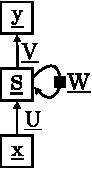
\includegraphics[width=\textwidth]{img/rnn.pdf}}
		\end{minipage}	
		\hspace{0.6cm}
		\begin{minipage}{0.6\textwidth}
		
		\slidesonly{
		\begin{textblock}{10}(5.0,3.5)
			\only<1> {\small define $s_i^{(t)}$ and $y_k^{(t)}$:}
			\only<2> {\small switch from element-wise notation to vector notation}
		\end{textblock}
		}
			\begin{eqnarray*}
			\only<1>{
				s_i^{(t)} &=& \tanh \Big({\smallsum{k=1}{N} U_{ik} \, x_k^{(t)}} 
						{ + \smallsum{j=1}{H}  W_{ij} \, s_j^{(t-1)}}
						+ b^\mathrm{s}_i \Big) \,,
						\\
				y_k^{(t)} &=& f\Big({\smallsum{j=1}{H} 
						V_{kj} \, s_j^{(t)}} + b^\mathrm{y}_k\Big) \,,\\[0.7cm]
					\;\text{e.g.}\;f(\cdot) &:=& \text{e.g. } \mathrm{softmax}(\cdot) \text{ for classification}\\
					}
			\only<2>{
				\vec s^{(t)} &=& \tanh\Big({\vec U \, \vec x^{(t)}} 
						{ + \vec W \, \vec s^{(t-1)}}
						+ \vec b^\mathrm{s} \Big) \,,
						\\
				\vec y^{(t)} &=& f\Big({\vec V \, s^{(t)}} + \vec b^\mathrm{y}\Big) \,,\\[0.7cm]
					\;\text{e.g.}\;f(\cdot) &:=& \text{e.g. } \mathrm{softmax}(\cdot) \text{ for classification}\\
					}
			\end{eqnarray*}
		\end{minipage}
	\end{minipage}
\end{frame}

\newpage

\subsection{Training RNNs}
\subsubsection{Using the chain rule}

% ------------------------------------------------------------------------------
\begin{frame}\frametitle{\subsecname: \subsubsecname}
\slidesonly{
	\begin{minipage}{\textwidth} \hspace{5mm}
		\includegraphics<1->[height=4cm]{img/rnn.pdf}
		\hspace{12mm}
		%\includegraphics<2>[height=4cm]{img/rnn_unfolded.pdf}
		%\includegraphics<2>[height=4cm]{img/rnn_unfolded_backprop.pdf}
	\end{minipage}
	\vspace{1mm}
}
	\begin{itemize}
		\item<1-> cost function $e^{(\alpha,t)}$ for time 
				step $t$ of training sequence $\alpha$ 
			\vspace{-1mm}
			$$
				E^T = \smallfrac{1}{p} \sum\limits_{\alpha=1}^p
				\smallfrac{1}{n_\alpha}\smallsum{t=1}{n_\alpha} e^{(\alpha,t)} \,,
				\quad \text{for training set} \quad 
				\Big\{ \{ \vec x^{(\alpha,t)}, \vec y^{(\alpha,t)} 
					\}_{t=1}^{n_\alpha}\Big\}_{\alpha=1}^{p}
			$$
		\vspace{-1mm}
		\item<2-> gradient computation using the chain rule%by unfolding the network in time 
		\vspace{1mm}
		\item<2-> computational complexity: $\Set O(H^2)$, i.e. quadratic in the number of recurrent weights
		%\item<3-> both $\color{blue}\vec h^{(t)}$ and 
		%		$\color{darkgreen}\vec h^{(t-1)}$ depend on $\vec W$ 
		%		and $\vec U$ ($\leadsto \Set O(n^2)$):
		%	$$
		%		\frac{\partial {\color{blue}h_k^{(t)}}}{\partial W_{ij}}
		%		\quad=\quad 
		%		\Big(f'\big( \vec U \, \vec x^{(t)} 
		%			+ \vec W \, {\color{darkgreen}\vec h^{(t-1)}}
		%			+ \vec b \big) \Big)_k
		%		\cdot \Big( I_{ki} \, {\color{darkgreen}h_j^{(t-1)}} 
		%			+ \smallsum{l}{} W_{kl} 
		%			\smallfrac{\partial {\color{darkgreen}h_l^{(t-1)}}}%
		%				{\partial W_{ij}} \Big)
		%	$$
	\end{itemize}
	\vspace{-2mm}
	\blfootnote{\hfill \citep[for details see][]{Williams95}}
\end{frame}


\subsubsection{Using Backpropagation through time (BPTT)}

% ------------------------------------------------------------------------------
\begin{frame}\frametitle{\subsubsecname}
	\begin{minipage}{\textwidth} \hspace{5mm}
    \mode<presentation>{
		\includegraphics<1->[height=4cm]{img/rnn.pdf}
		\hspace{12mm}
		\includegraphics<1,3>[height=4cm]{img/rnn_unfolded_untie.pdf}
		\includegraphics<2>[height=4cm]{img/rnn_unfolded_bptt.pdf}
        }
    \mode<article>{
		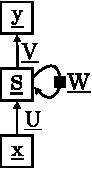
\includegraphics[height=4cm]{img/rnn.pdf}
		\hspace{10mm}
		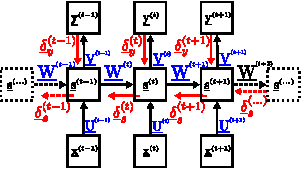
\includegraphics[height=4cm]{img/rnn_unfolded_bptt.pdf}
    }
	\end{minipage}
	\vspace{1mm}
	\begin{itemize}
		\item<1-> assume all unfolded weights, 
				e.g.~$\color{blue}\vec W^{(t)}$, are independent
		\vspace{1mm}
		\item<2-> compute gradients of deep MLP with backpropagation 
				($ \Set O(n)$, where $n$ is the total number of all weights in the unrolled network)
		\vspace{1mm}
		\item<3-> average all computed gradients, i.e.  
				${\color{blue} \frac{\partial e^{(\alpha,t)}}%
				{\partial \vec W^{(\alpha,\tau)}}}$, 
				for weight update:\\
				\vspace{-1mm}
			$$ \hspace{-5mm}
				\Delta \vec W \;\; = \;\;
					-\eta \, \smallfrac{\partial E^T}{\partial \vec W}
				\;\;=\;\; -\smallfrac{\eta}{p} 
					\smallsum{\alpha=1}{p} \smallfrac{1}{n_{\alpha}}  \smallsum{t=1}{n_{\alpha}}
					\smallfrac{\partial e^{(\alpha, t)}}{\partial \vec W}
				\;\;\approx\;\; -\smallfrac{\eta}{p}
					\smallsum{\alpha=1}{p} \smallfrac{1}{n_{\alpha}} \smallsum{t=1}{n_{\alpha}} \smallfrac{1}{t} \smallsum{\tau=1}{t}
					{\color{blue} \smallfrac{\partial e^{(\alpha,t)}}%
						{\partial \vec W^{(\alpha,\tau)}}}
			$$
	\end{itemize}
\end{frame}

\begin{frame}
\mode<presentation>{
	\begin{minipage}{\textwidth} \hspace{5mm}
		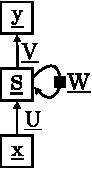
\includegraphics[height=4cm]{img/rnn.pdf}
		\hspace{12mm}
		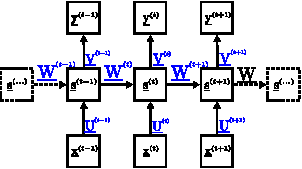
\includegraphics[height=4cm]{img/rnn_unfolded_untie.pdf}
	\end{minipage}
	\vspace{1mm}
	\begin{itemize}
		\item[]
			$$ \hspace{-5mm}
				\Delta \vec W
				\;\;\approx\;\; -\smallfrac{\eta}{p}
					\smallsum{\alpha=1}{p} \smallfrac{1}{n_{\alpha}} \smallsum{t=1}{n_{\alpha}} \smallfrac{1}{t} \smallsum{\tau=1}{t}
					{\color{blue} \smallfrac{\partial e^{(\alpha,t)}}%
						{\partial \vec W^{(\alpha,\tau)}}}
			$$
	\end{itemize}
	}
The backpropagation algorithm provides an \emph{exact} computation of the gradients.
However, 
since BPPT involves unfolding the weights (unrolling the network), this leads to an \emph{approximation of the gradients}.
\end{frame}
